\section{Selection on Kin Cooperating Group Structure}

\begin{frame}
\begin{itemize}
\item expect transition to occur
\item scalable
\item no simulation of ``realistic'' physics, abstract instead
\end{itemize}
\end{frame}

\begin{frame}{Resource Collection}
\begin{itemize}
\item need to anticipate
\item need to activate
\item communication with neighbors
\end{itemize}
\end{frame}

\begin{frame}{Channels, Signals, \& Resource}
\begin{itemize}
\item register into explicit cooperating groups called channels
\end{itemize}
\end{frame}

\begin{frame}{Channels, Signals, \& Resource}

\foreach \n in {1,...,10}{%
\includegraphics<\n>[width=\textwidth]{explanatory/explanatory-\n.pdf}%
}%

\end{frame}

\begin{frame}{Signals \& Resource}
  \vspace{4ex}
  \begin{figure}
\begin{columns}
\begin{column}{0.5\textwidth}
    \foreach \n in {1,...,12}{%
    \includegraphics<\n>[width=\textwidth]{small_res/frame-\n.png}%
    }%
\end{column}
\begin{column}{0.5\textwidth}
    \foreach \n in {1,...,12}{%
    \includegraphics<\n>[width=\textwidth]{small_sig/frame-\n.png}%
    }%
\end{column}
\end{columns}%
\begin{columns}
\begin{column}{0.5\textwidth}
\begin{subfigure}[b]{\textwidth}
  \caption{resource}
\end{subfigure}
\end{column}
\begin{column}{0.5\textwidth}
\begin{subfigure}[b]{\textwidth}
\caption{activation-quiescence signals}
\end{subfigure}
\end{column}
\end{columns}
\caption{Co-visualization of same-channel signaling and resource distribution.}
\end{figure}

\end{frame}

\begin{frame}{Channel Inheritance}
  \vspace{8ex}
  \begin{figure}
\begin{columns}
  \begin{column}{0.5\textwidth}
    \colorbox{extralightgray}{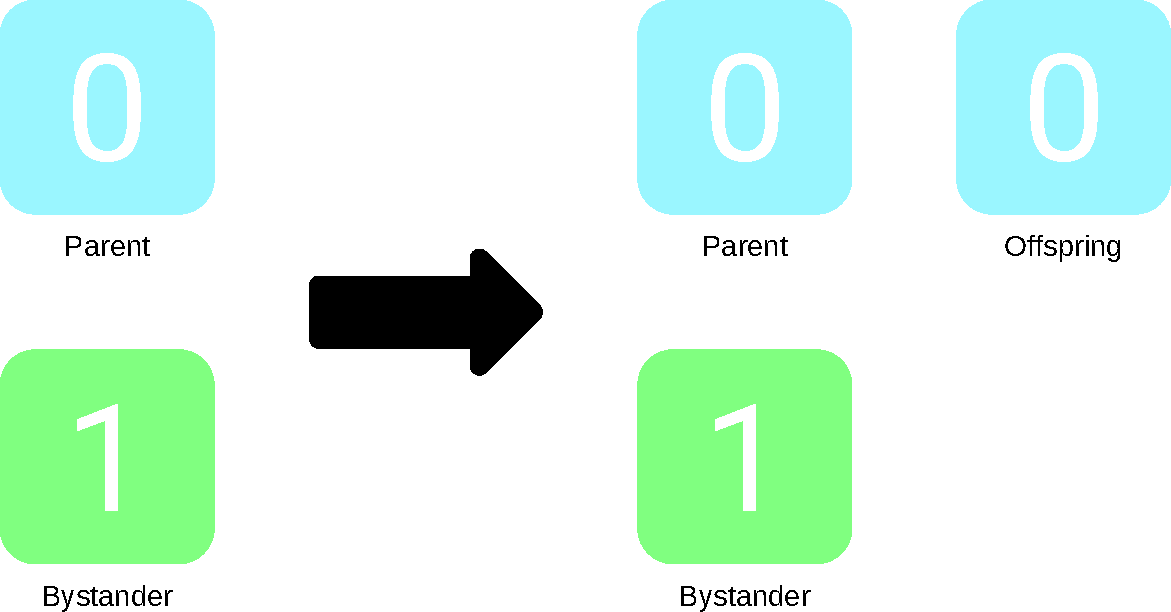
\includegraphics[width=\textwidth]{same_channel_offspring}}
  \end{column}%
  \begin{column}{0.5\textwidth}
    \colorbox{extralightgray}{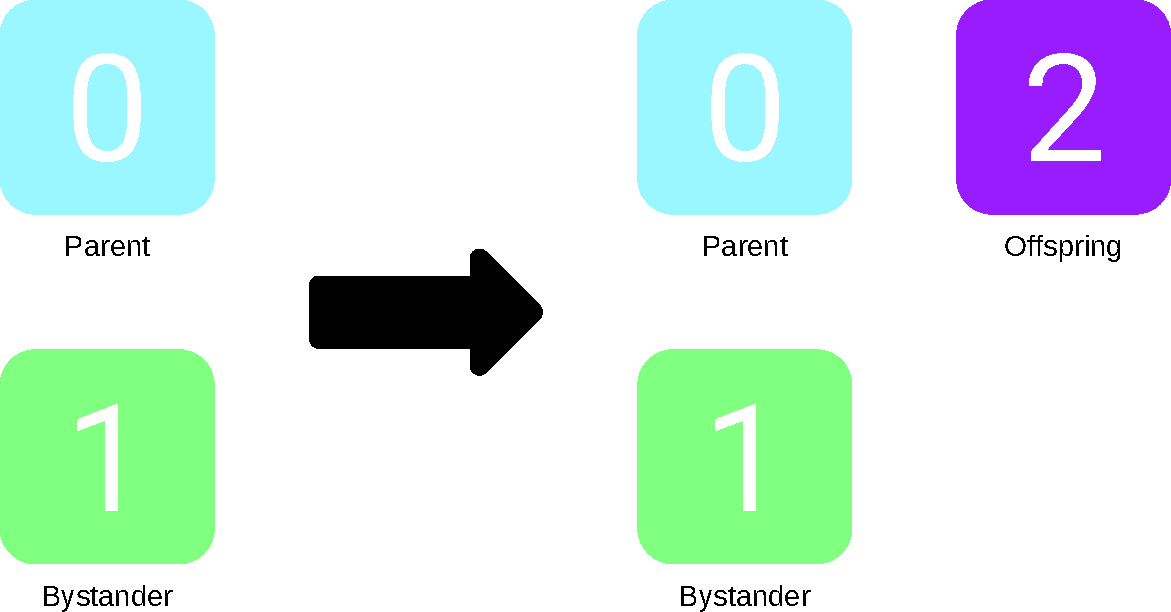
\includegraphics[width=\textwidth]{new_channel_offspring}}
  \end{column}%
\end{columns}%
\begin{columns}
  \begin{column}{0.5\textwidth}
    \begin{subfigure}[b]{\textwidth}
    \caption{Offspring inherits channel ID from parent.}
    \end{subfigure}
  \end{column}%
  \begin{column}{0.5\textwidth}
    \begin{subfigure}[b]{\textwidth}
    \caption{Offspring assigned new, unique channel ID.}
    \end{subfigure}
  \end{column}%
\end{columns}%
\caption{The two possible channel inheritance outcomes.}
\end{figure}

\end{frame}

\begin{frame}{Excluded Channel Dynamics}
  \vspace{6.6ex}
  \begin{figure}
\begin{columns}
  \begin{column}{0.5\textwidth}
\colorbox{extralightgray}{\hspace{0.136\textwidth}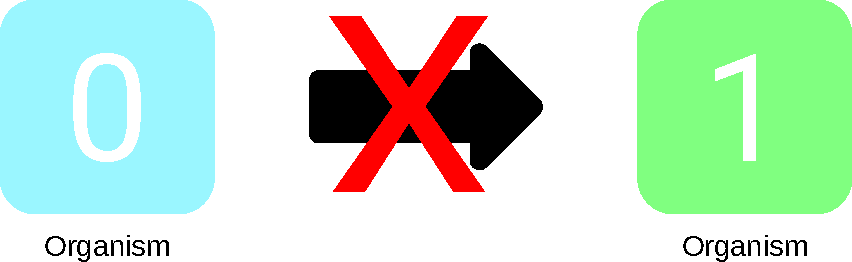
\includegraphics[width=0.728\textwidth,trim= 0 -83 0 -83]{plastic_channel}\hspace{0.136\textwidth}}
  \end{column}%
  \begin{column}{0.5\textwidth}%
\colorbox{extralightgray}{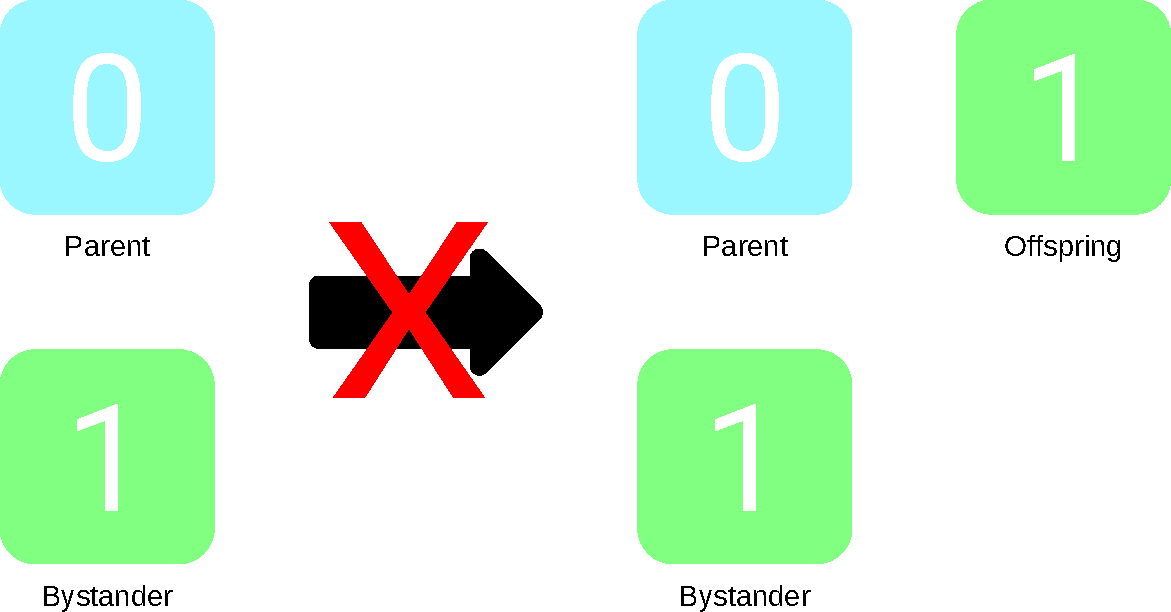
\includegraphics[width=\textwidth]{channel_collision_offspring}}
  \end{column}
\end{columns}%
\begin{columns}
  \begin{column}{0.5\textwidth}
    \begin{subfigure}[b]{\textwidth}
    \caption{during-lifetime channel change}
    \end{subfigure}
  \end{column}
  \begin{column}{0.5\textwidth}
    \begin{subfigure}[b]{\textwidth}
    \caption{non-inherited channel match\footnotemark}
    \end{subfigure}
  \end{column}
\end{columns}
\caption{Illustration of excluded channel dynamics.}
\end{figure}
\footnotetext{infrequent, non-inducible}

\end{frame}

\begin{frame}{Intuition}
key idea: selection on regulation of same-channel group size \& shape
\begin{itemize}
  \item too small: low resource-collection rate
  \item too big: net negative resource collection due to erroneous activation
\end{itemize}

more generally speaking,

Selection on Kin Cooperating Group Structure

\end{frame}
